\subsection{Loop Blocking}

Loop blocking is a technique to improve the memory access and data re-use, and thereby reduce the cache misses. To perform this, the matrices is essentially cut into smaller blocks, which are then solved, where more of the information can be reused, since it is already available in the cache. By implementing loop blocking, we intend to compare the performance of the new blocked loop function with the best performing permutation, which is mkn. The function prototype is almost identical to the earlier used with the new addition, that it takes a specified integer bs as an argument.

\begin{lstlisting}[language=C++, caption=Blocked blk Prototype]
void matmult_blk(int m, int n, int k, double ** A, double ** B, double ** C, int bs)
\end{lstlisting}

To implement the blocking itself for arbitrarily sized matrices, we introduce 3 blocking size variables in the loop for each dimension. Since the blocking is performed for each dimension, we need six nested loops. The first three are the blocking loops to increases in increments of the blocking size. These include an if conditional, in the case, when the specific dimension is not dividable by the block variable. In the last run of the loop, there may be a case where the blocking size is actually bigger than the missing number of loop variables (dimension size - loop variable), in which case the bs variable is set equal to the number of missing rowx/columns for that dimension. This secures that no segmentation error occur.\\

The three inner loops basically runs over the according block sizes for the three dimension variables.

\begin{lstlisting}[language=C++, caption=Blocked Loop Function]
int bsi=bs;
int bsj=bs;
int bsl=bs;

for(int i1 = 0; i1 < m;i1+=bsi){
	if(m-i1 < bs) {bsi=m-i1;
	}
	for(int l1 = 0; l1 < k;l1+=bsl){
		if(k-l1 < bs) {bsl=k-l1;
		}
		for(int j1 = 0; j1 < n;j1+=bsj){
			if(n-j1 < bs) {bsj=n-j1;
			}
			for(int i2 = 0; i2 < bsi; i2++){	
				for(int l2 = 0; l2 < bsl;l2++){	
					for(int j2 = 0; j2 < bsj; j2++){	
						C[i1+i2][j1+j2] += 
						A[i1+i2][l1+l2]*B[l1+l2][j1+j2];
					}
				}
			}
		}
	}
}
\end{lstlisting}

It would also be easy to implement different initial block sizes to experiment with different block dimensions and structures, i.e. a rectangle, but this is however not researched in our report. It could also be interesting to look into how the blocking perform with different type of rectangles, but these experiments have been performed on square matrices.


\subsubsection{Block Performance and Comparison}

Since the optimal blocking size varies with different matrix dimension, we seek to determine a good overall block size to use the same parameter for a memory footprint comparison with the best permutation mkn and the library function.\\
An experiment with varying block sizes are run for a 2000x2000, which is displayed in figure \ref{fig:optblock}. The different blocksizes found can then also be compared to the L1, L2 and L3 caches. So the variations however small, clearly show the advantage of the correct block size and how it suits the different cache sizes. The peak right before the L2 cache is with a block size of 100. This block size is then chosen to use for the rest of the experiments.

\begin{figure}[h!] 
	\begin{center}
		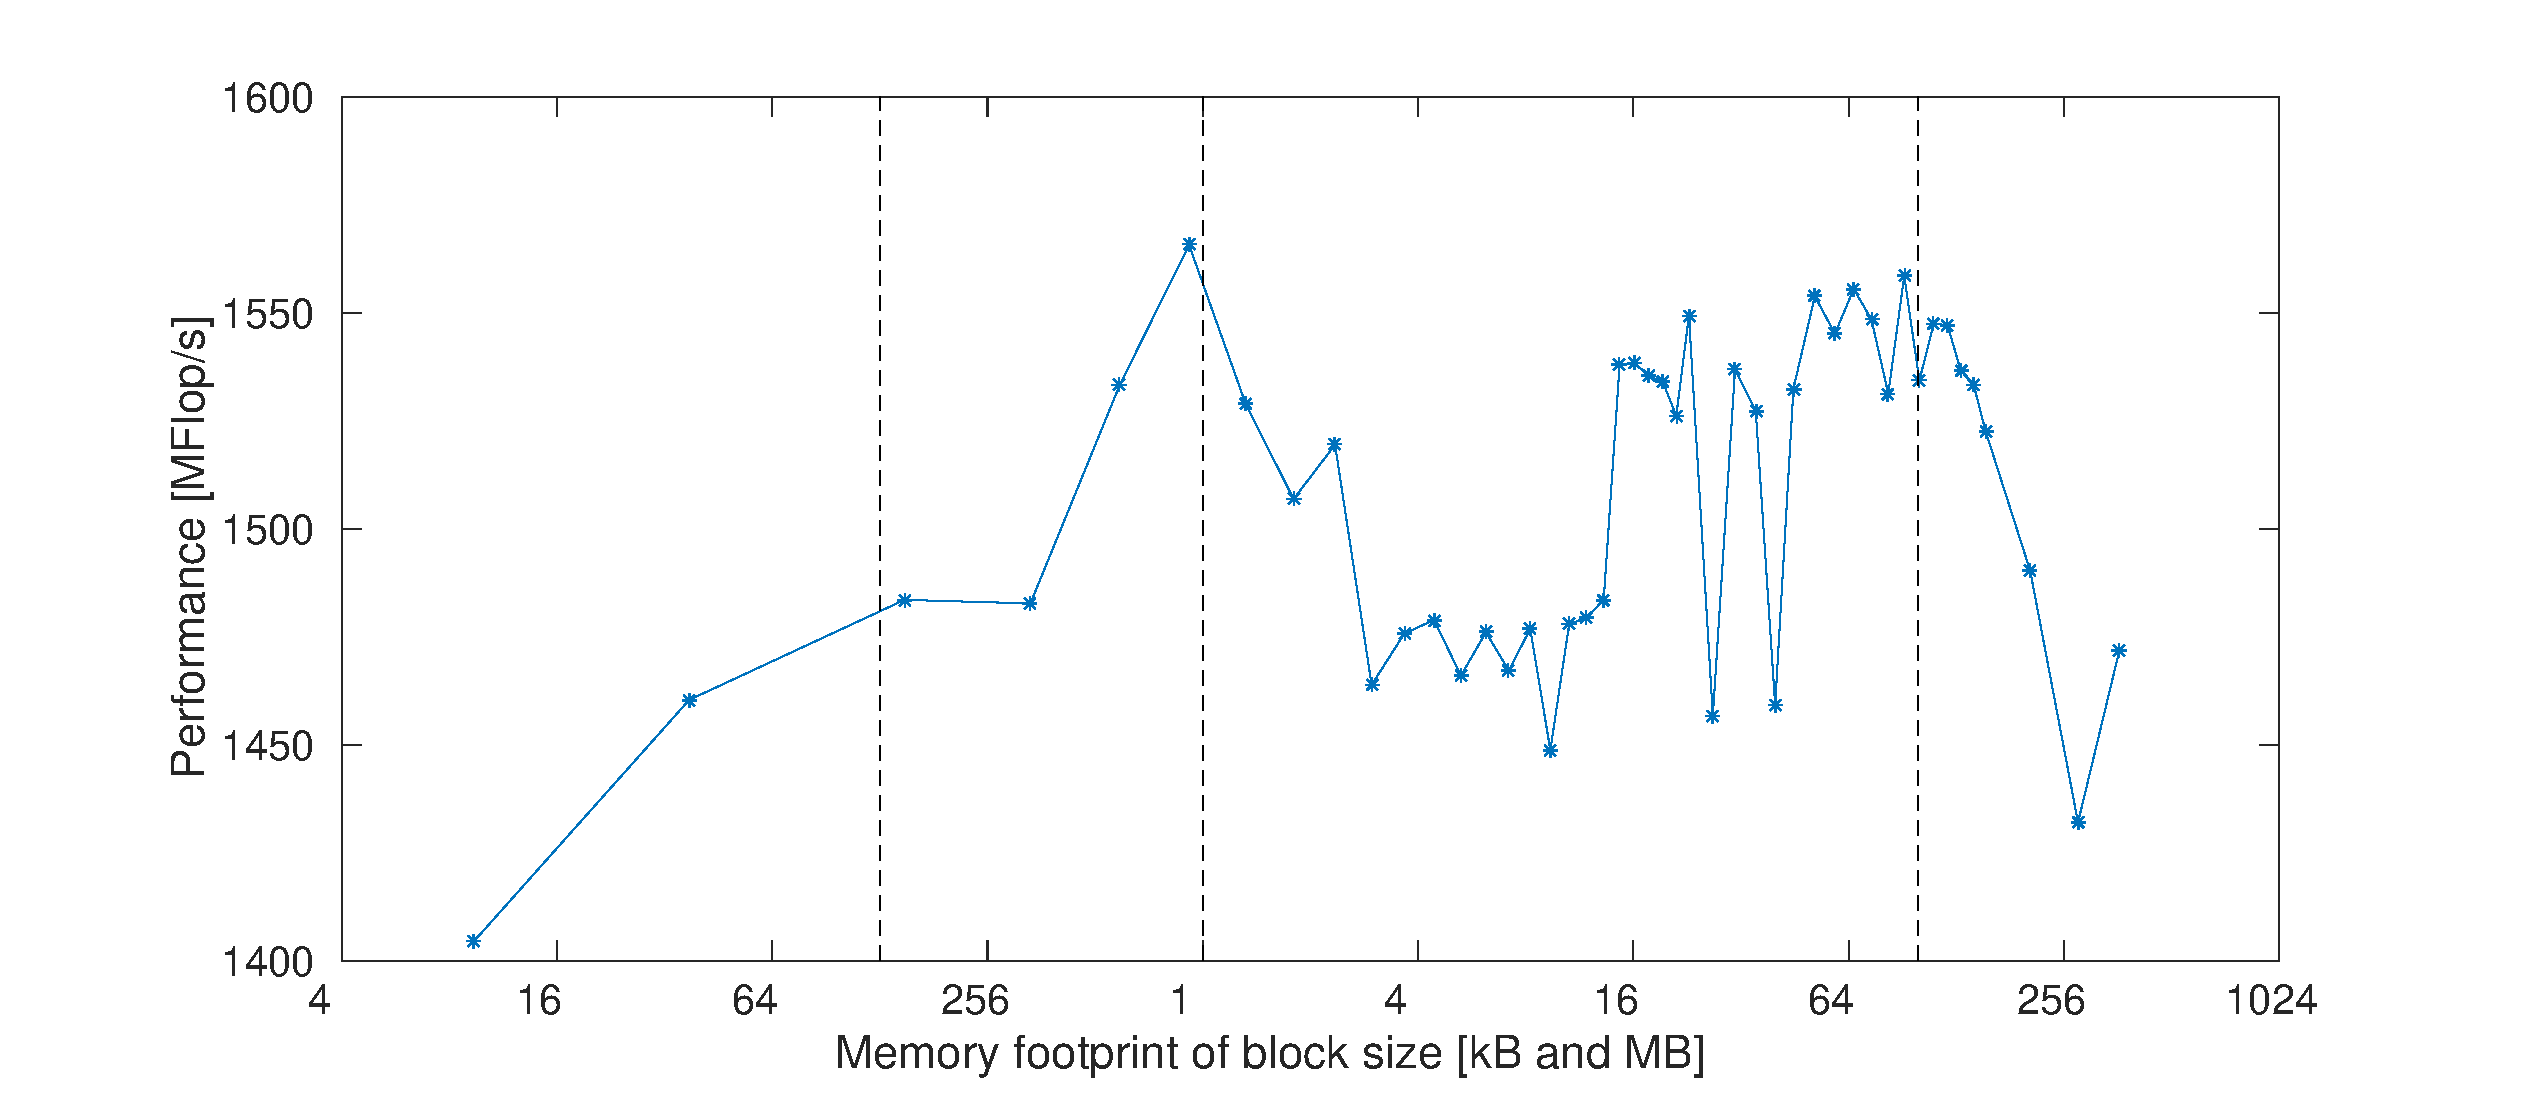
\includegraphics[width=1.1 \textwidth]{fig/optimalBlock.eps} 
		\caption{d}
		\label{fig:optblock}
	\end{center}
\end{figure}

The memory footprint for the blk and mkn is created, using a blocking size of 100. It should be noted, that the blk function is using the same loop structure as mkn. There are multiple factors in play here, and they perform almost identical with matrices of small sizes, but the mkn function do however perform better. This is probably caused by the additional loops and if statements in the blocking function. It can be seen that mkn performs surprisingly well for matrices of bigger sizes, and the blk function falls of a bit around 4 MB. The decent performance of the mkn function is partly caused by the Sun Studio compiler, which is very optimized already. Furthermore, the mkn permutation is already performing the calculation in the best suitable way memory wise. The mkn function do however start to fall off in MFlop/s, once the matrix sizes increases above the L3 cache size, which makes sense, since there is a penalty on accessing the RAM, whereas the blk function largely avoids that, and does not face the same downward trend. If we had run the experiment for bigger matrix sizes, the result may very well have been that the mkn function would continue to fall of, and the blk function would perform better on matrices of sizes above 1 GB.

\begin{figure}[h!] 
	\begin{center}
		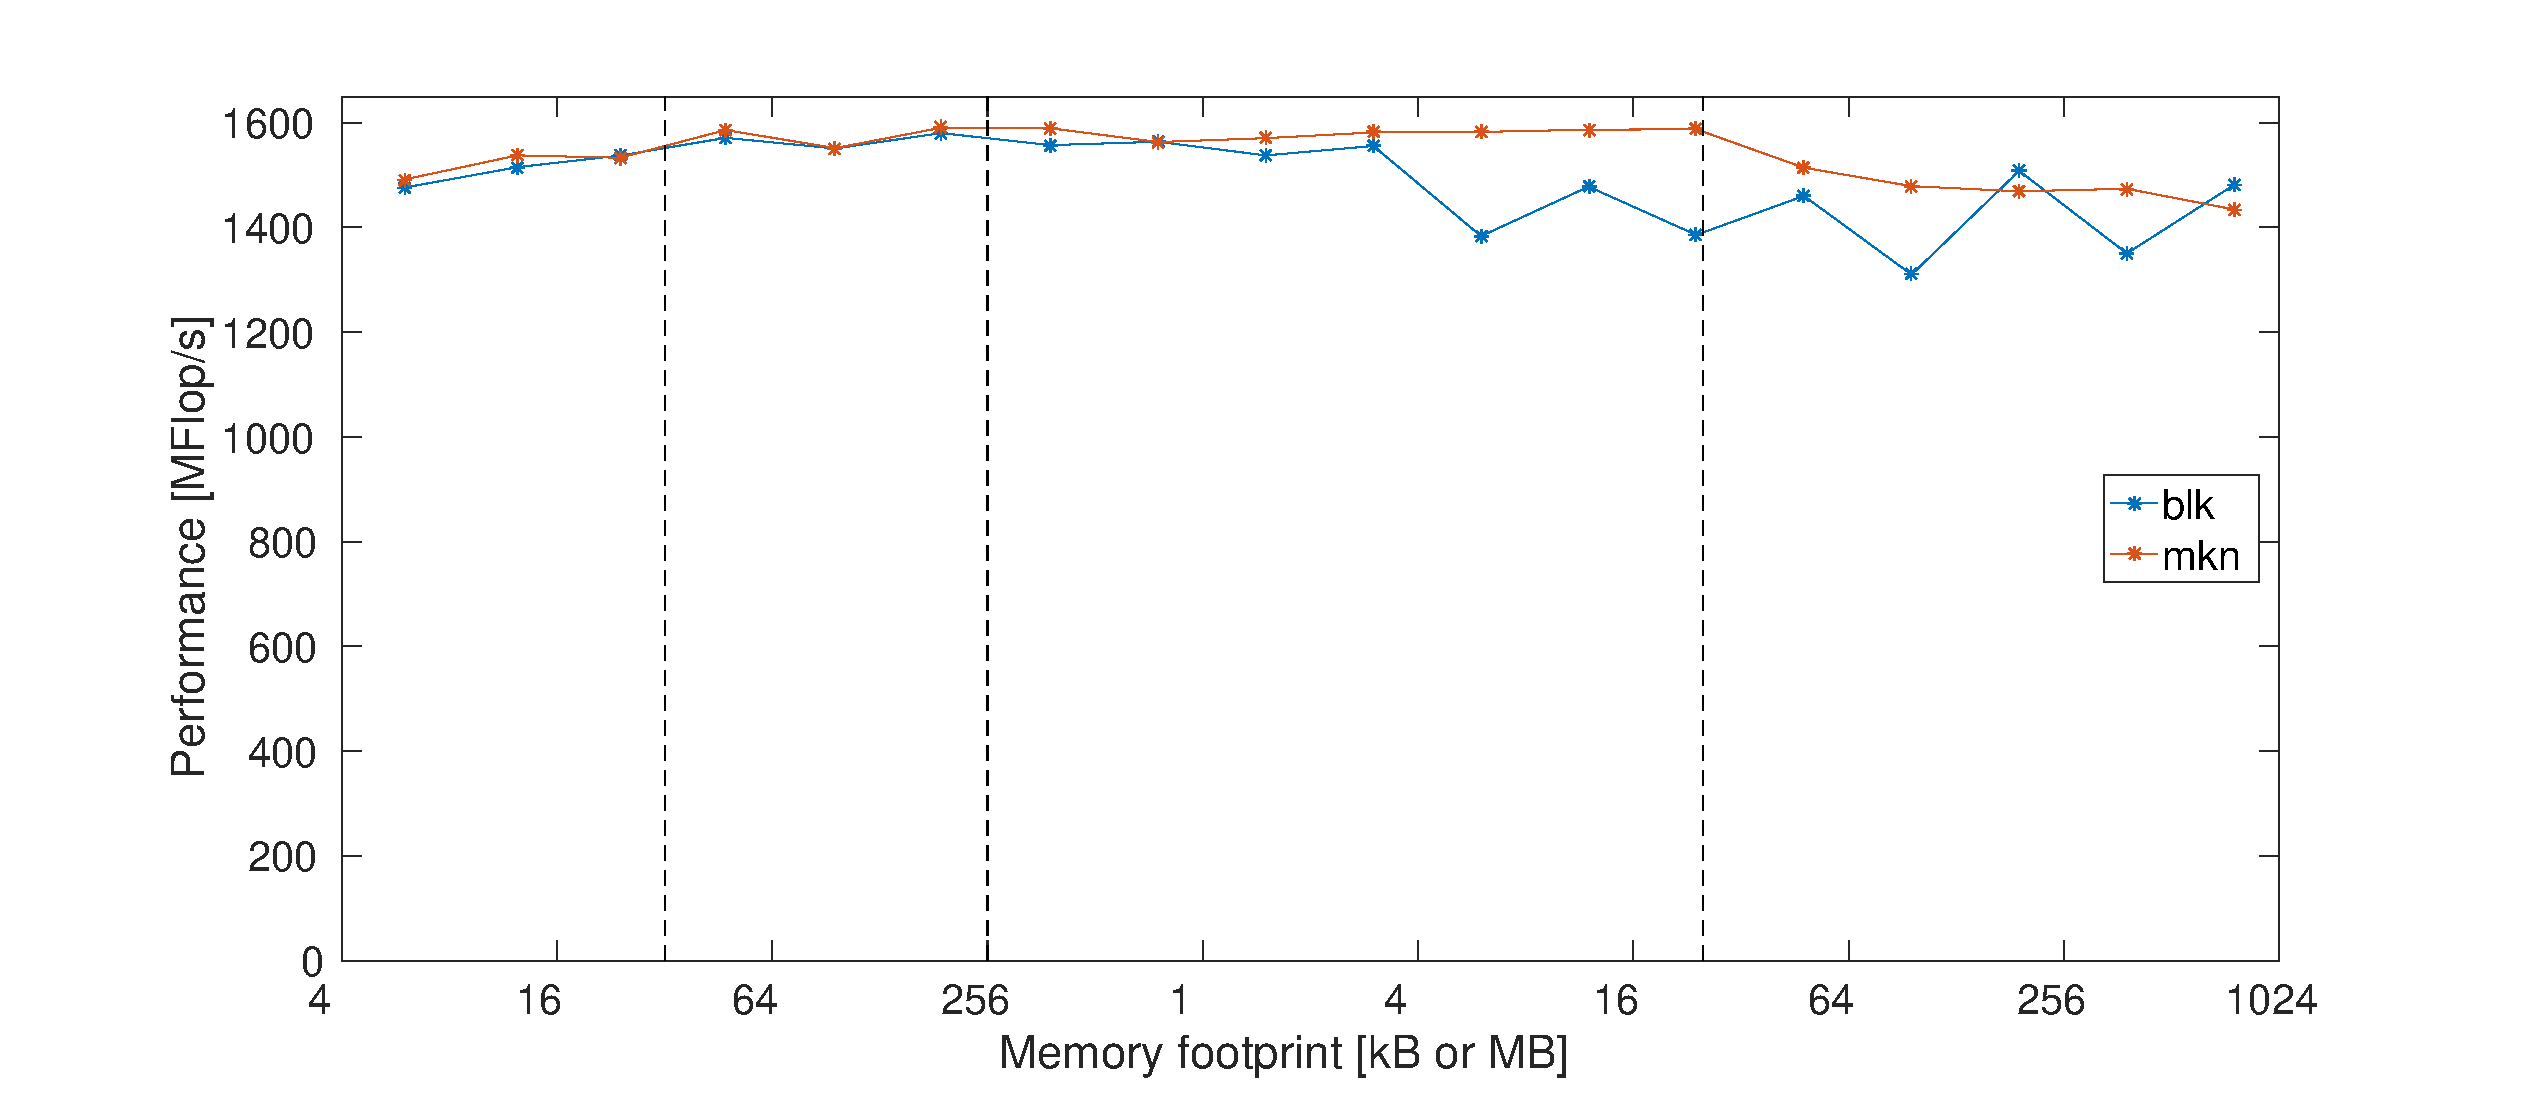
\includegraphics[width=1.1 \textwidth]{fig/permGraph_blk_mkn.eps} 
		\caption{The memory footprint of the blk and mkn functions.}
		\label{fig:mknblk}
	\end{center}
\end{figure}


We are now ready to compare the blk function with the library function DGEMM, but we quickly realize that these are not in the same league since the MFlop/s of the lib function is mostly above 20000. The performance of the library function is far superior to our own novice functions.